\documentclass[a4paper]{article}
\ProvidesPackage{bkthesis}
\usepackage{vntex}
\usepackage{a4wide,amssymb,epsfig,latexsym,array,hhline,fancyhdr}
\usepackage[normalem]{ulem}
%\usepackage{soul}

\usepackage[makeroom]{cancel}
\usepackage{amsmath}
\usepackage{amsthm}
\usepackage{multicol,longtable,amscd}
\usepackage{diagbox}%Make diagonal lines in tables
\usepackage{booktabs}
\usepackage{alltt}
\usepackage[framemethod=tikz]{mdframed}% For highlighting paragraph backgrounds
\usepackage{caption,subcaption}

\usepackage{lastpage}
\usepackage[lined,boxed,commentsnumbered]{algorithm2e}
\usepackage{enumerate}
\usepackage{color}
\usepackage{graphicx}							% Standard graphics package
\usepackage{array}
\usepackage{tabularx, caption}
\usepackage{multirow}
\usepackage{multicol}
\usepackage{rotating}
\usepackage{graphics}
\usepackage{geometry}
\usepackage{setspace}
\usepackage{epsfig}
\usepackage{tikz}
\usepackage{float}
\usepackage{listings}
\usepackage{lscape} % hoặc pdflscape nếu dùng pdf output
\usetikzlibrary{arrows,snakes,backgrounds}
\usepackage[unicode]{hyperref}
\hypersetup{urlcolor=blue,linkcolor=black,citecolor=black,colorlinks=true} 
%\usepackage{pstcol} 								% PSTricks with the standard color package

\usepackage{listings}

\usepackage{color} % tô màu cho code


\definecolor{dkgreen}{rgb}{0,0.6,0}
\definecolor{gray}{rgb}{0.5,0.5,0.5}
\definecolor{mauve}{rgb}{0.58,0,0.82}

\lstset{frame=tb,
  language=Python,
  aboveskip=3mm,
  belowskip=3mm,
  showstringspaces=false,
  columns=flexible,
  basicstyle={\small\ttfamily},
  numbers=none,
  numberstyle=\tiny\color{gray},
  keywordstyle=\color{blue},
  commentstyle=\color{dkgreen},
  stringstyle=\color{mauve},
  breaklines=true,
  breakatwhitespace=true,
  tabsize=3
}







\usepackage[normalem]{ulem}

\newtheorem{theorem}{{\bf Định lý}}
\newtheorem{property}{{\bf Tính chất}}
\newtheorem{proposition}{{\bf Mệnh đề}}
\newtheorem{corollary}[proposition]{{\bf Hệ quả}}
\newtheorem{lemma}[proposition]{{\bf Bổ đề}}
\theoremstyle{definition}
\newtheorem{exer}{Bài toán}

\def\thesislayout{	% A4: 210 × 297
	\geometry{
		a4paper,
		total={160mm,240mm},
		left=30mm,
		top=30mm,
	}
}
\thesislayout

%\usepackage{fancyhdr}
\setlength{\headheight}{40pt}
\pagestyle{fancy}
\fancyhead{} % clear all header fields
\fancyhead[L]{
 \begin{tabular}{rl}
    \begin{picture}(25,15)(0,0)
    \put(0,-8){
\includegraphics[width=8mm, height=8mm]{image/hcmut.png}}
    %\put(0,-8){\epsfig{width=10mm,figure=hcmut.eps}}
   \end{picture}&
	%
\includegraphics[width=8mm, height=8mm]{hcmut.png} & %
	\begin{tabular}{l}
		\textbf{\bf \ttfamily Trường Đại Học Bách Khoa Tp.Hồ Chí Minh}\\
		\textbf{\bf \ttfamily Khoa Khoa Học \& Kỹ Thuật Máy Tính}
	\end{tabular} 	
 \end{tabular}
}
\fancyhead[R]{
	\begin{tabular}{l}
		\tiny \bf \\
		\tiny \bf 
	\end{tabular}  }
\fancyfoot{} % clear all footer fields
\fancyfoot[L]{\scriptsize \ttfamily Kiến Trúc Máy Tính - Năm học 2023-2024}
\fancyfoot[R]{\scriptsize \ttfamily Trang {\thepage}/\pageref{LastPage}}
\renewcommand{\headrulewidth}{0.3pt}
\renewcommand{\footrulewidth}{0.3pt}


%%%
\setcounter{secnumdepth}{4}
\setcounter{tocdepth}{3}
\makeatletter
\newcounter {subsubsubsection}[subsubsection]
\renewcommand\thesubsubsubsection{\thesubsubsection .\@alph\c@subsubsubsection}
\newcommand\subsubsubsection{\@startsection{subsubsubsection}{4}{\z@}%
                                     {-3.25ex\@plus -1ex \@minus -.2ex}%
                                     {1.5ex \@plus .2ex}%
                                     {\normalfont\normalsize\bfseries}}
\newcommand*\l@subsubsubsection{\@dottedtocline{3}{10.0em}{4.1em}}
\newcommand*{\subsubsubsectionmark}[1]{}
\makeatother

% \everymath{\color{blue}}
%make in-line maths symbols blue to read/check easily

\sloppy
\captionsetup[figure]{labelfont={small,bf},textfont={small,it},belowskip=-1pt,aboveskip=-9pt}
%space remove between caption, figure, and text
\captionsetup[table]{labelfont={small,bf},textfont={small,it},belowskip=-1pt,aboveskip=7pt}
%space remove between caption, table, and text

%\floatplacement{figure}{H}%forced here float placement automatically for figures
%\floatplacement{table}{H}%forced here float placement automatically for table
%the following settings (11 lines) are to remove white space before or after the figures and tables
%\setcounter{topnumber}{2}
%\setcounter{bottomnumber}{2}
%\setcounter{totalnumber}{4}
%\renewcommand{\topfraction}{0.85}
%\renewcommand{\bottomfraction}{0.85}
%\renewcommand{\textfraction}{0.15}
%\renewcommand{\floatpagefraction}{0.8}
%\renewcommand{\textfraction}{0.1}
\setlength{\floatsep}{5pt plus 2pt minus 2pt}
\setlength{\textfloatsep}{5pt plus 2pt minus 2pt}
\setlength{\intextsep}{10pt plus 2pt minus 2pt}

\thesislayout

\begin{document}

\begin{titlepage}
\begin{center}
ĐẠI HỌC QUỐC GIA THÀNH PHỐ HỒ CHÍ MINH \\
TRƯỜNG ĐẠI HỌC BÁCH KHOA \\
KHOA KHOA HỌC \& KỸ THUẬT MÁY TÍNH 
\end{center}

\vspace{1cm}

\begin{figure}[h!]
\begin{center}

\includegraphics[width=5cm]{image/hcmut.png}
\end{center}
\end{figure}

\vspace{1cm}


\begin{center}
\begin{tabular}{c}
\multicolumn{1}{l}{\textbf{{\Large \hspace{2cm}KIẾN TRÚC MÁY TÍNH (CO2008)}}}\\
~~\\
\hline
\\
\textbf{\Large Bài tập lớn} \\
\textbf{\Large Kiến trúc tập lệnh } \\
\textbf{\Large Đề 2} \\
\\
\hline
\end{tabular}
\end{center}

\vspace{0.5cm}

\begin{table}[h]
\begin{tabular}{rrl}

\hspace{3.5 cm} & \color{black}{GVHD:} & \color{black}{NGUYỄN XUÂN MINH}\\ 

\hspace{0.5 cm} & \color{black}{SV thực hiện:} & \color{black}{TRẦN MINH DƯƠNG- 2310609}\\ &\color{black} &\color{black}{PHẠM CÔNG VÕ - 2313946}\\

\hspace{3.5 cm} & \color{black}{Lớp:} & \color{black}{L02}\\
&\color{black}{Nhóm:} &\color{black}{21}\\

\end{tabular}
\end{table}
\vspace{5cm}
\begin{center}
{\footnotesize \hspace{1cm} \large Tp. Hồ Chí Minh, Tháng 5/2025}
\end{center}
\end{titlepage}


%\thispagestyle{empty}
%%


%%

\newpage
% -	Lời cảm ơn/ Lời ngỏ
\Large \textbf{Lời Cảm Ơn} \small \\

\large Đầu tiên, nhóm chúng em xin được gửi lời cảm ơn đến giảng viên là thầy Nguyễn Xuân Minh đã giúp
nhóm thực hiện bài tập lớn này. Nhờ sự giúp đỡ tận tình của quý thầy, chúng em đã vượt qua những
khúc mắc, khó khăn trong suốt quá trình thực hiện bài tập, từ đó hoàn thành đúng tiến độ của môn học
và cho ra sản phẩm chất lượng.
Ngoài ra, không thể không nhắc đến sự quan tâm giúp đỡ của các anh chị, các bạn sinh viên trong
cộng đồng sinh viên trường Đại học Bách Khoa nói riêng và ĐHQG-HCM nói chung, những đóng góp
tolớn của các anh, chị và các bạn đã giúp chúng em nắm chắc hơn cách sử dụng kiến trúc tập lệnh MIPS
mà nhóm chỉ mới gần đây được tiếp cận trong quá trình theo học ở môi trường Đại học.
Cuối cùng, nhóm chúng em xin gửi lời cảm ơn một lần nữa đến các tập thể, cá nhân đã giúp đỡ và
truyền cảm hứng cho nhóm trong suốt quá trình thực hiện dự án bài tập lớn này. 

\newpage
\tableofcontents
\newpage
\listoffigures
\newpage
% \section{Lời Cảm Ơn}
\section{Giới thiệu đề tài}

\subsection{Giới thiệu về MIPS}
\indent MIPS - Microprocessor without Interlocked Pipeline Stages - là kiến trúc bộ tập lệnh RISC phát triển
bởi MIPS Technologies. Ban đầu kiến trúc MIPS là 32bit, và sau đó là phiên bản 64 bit. Nhiều sửa đổi
của MIPS, bao gồm MIPS I, MIPS II, MIPS III, MIPS IV, MIPS V, MIPS32 và MIPS64. Phiên bản hiện
tại là MIPS32 và MIPS64.
\subsection{Đề bài 2:}
\textbf{Cộng 2 số thực chuẩn IEEE 754 chính xác đơn.
Viết chương trình thực hiện phép cộng 2 số thực chuẩn IEEE 754 chính xác đơn mà không dùng
các lệnh tính toán số thực của MIPS. Dữ liệu đầu vào đọc từ file lưu trữ dạng nhị phân trên đĩa
FLOAT2.BIN (2 trị x 4 bytes = 8 bytes). 
}\\\\
\textbf{\textit{* Biểu diễn số thực trong máy tính theo chuẩn IEEE 754}}\\\\
Máy tính chỉ có khả năng lưu trữ và xử lý các tín hiệu dưới dạng nhị phân. Do đó, để biểu diễn một số thực trong máy tính, trước tiên chúng ta cần chuyển đổi số đó sang dạng nhị phân. Tuy nhiên, không thể áp dụng cách biểu diễn như đối với số nguyên, mà cần tuân theo một chuẩn riêng biệt – phổ biến nhất là chuẩn \textbf{IEEE 754}.
Chuẩn IEEE 754 quy định hai định dạng chính để biểu diễn số thực.
\begin{itemize}
    \item \textbf{Độ chính xác đơn (single precision)}: sử dụng 32 bit, bao gồm 1 bit dấu, 8 bit cho phần mũ và 23 bit cho phần trị (phần lẻ).
    \item \textbf{Độ chính xác kép (double precision)}: sử dụng 64 bit, bao gồm 1 bit dấu, 11 bit cho phần mũ và 52 bit cho phần trị.
\end{itemize}
\begin{figure}[!h]
    \centering 
    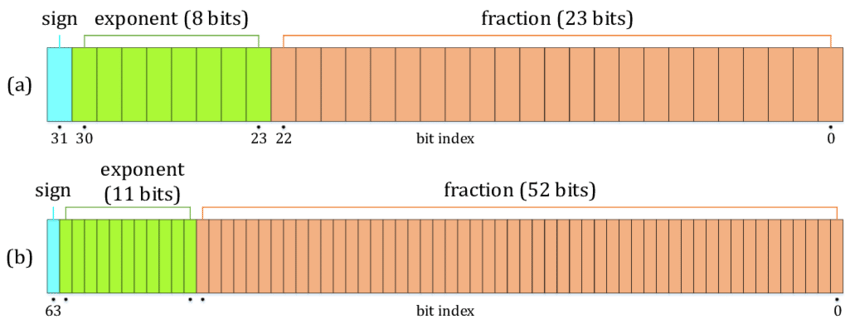
\includegraphics[width=0.8\textwidth]{image/IEEE Standard for Floating-Point Arithmetic (IEEE 754).png}
    \vspace{0.5cm} % khoảng cách sau caption (nếu muốn)
      \caption{ IEEE Standard for Floating-Point Arithmetic (IEEE 754)}
\end{figure}

Trước khi một số thực có thể được lưu trữ theo chuẩn IEEE 754, cần chuyển đổi số đó về \textbf{dạng chuẩn hóa}, tức là biểu diễn sao cho phần nguyên của số không chứa số 0 (ngoại trừ số 0 chính nó).\\

\textbf{\textit{* Thống kê số lượng lệnh R, I, J trong chương trình MIPS}}\\

Trong quá trình phát triển chương trình mô phỏng hợp ngữ MIPS, tổng số lệnh được sử dụng thuộc ba loại R, I và J được thống kê như sau:

\begin{table}[H]
\centering
\begin{tabular}{|c|c|}
\hline
\textbf{Loại lệnh} & \textbf{Số lượng} \\
\hline
R & 20 \\
\hline
I & 36 \\
\hline
J & 4 \\
\hline
\end{tabular}
\caption{Thống kê số lượng lệnh R, I, J sử dụng trong chương trình MIPS}
\end{table}


\section{Giải thuật}
\subsection{Hướng tiếp cận tổng quát}

Để thực hiện phép cộng (hoặc trừ) hai số thực biểu diễn theo chuẩn \textbf{IEEE 754}, ta cần tuần tự thực hiện các bước sau:

\begin{itemize}
    \item \textit{Bước 1: Chuẩn hóa các số} \\
    Chuyển hai số thực $X$ và $Y$ từ thanh ghi về dạng chuẩn hóa theo IEEE 754:
    \[
        X = 1.xxx\ldots x \times 2^{\text{exponent}_X - 127} \tag{1}
    \]
    \[
        Y = 1.yyy\ldots y \times 2^{\text{exponent}_Y - 127} \tag{2}
    \]
    \textit{Lưu ý:} Dãy bit $x$ hoặc $y$ gồm 23 bit, tương ứng với phần \textbf{fraction (mantissa)} trong chuẩn IEEE 754.

    \item \textit{Bước 2: Căn chỉnh số mũ} \\
    So sánh hai số mũ $\text{exponent}_X$ và $\text{exponent}_Y$. Dịch phải phần mantissa của số có số mũ nhỏ hơn cho đến khi cả hai số có cùng số mũ (tức là cùng cơ số $2^{\text{exponent} - 127}$).

    \item \textit{Bước 3: Thực hiện phép cộng/trừ} \\
    Sau khi đã căn chỉnh số mũ, thực hiện phép cộng hoặc trừ trên phần mantissa của hai số.

    \item \textit{Bước 4: Chuẩn hóa kết quả} \\
    Chuẩn hóa lại kết quả nếu cần thiết (ví dụ: nếu xảy ra tràn hoặc cần dịch trái để đưa về dạng chuẩn), sau đó mã hóa lại theo định dạng IEEE 754 để lưu trữ hoặc xuất kết quả.
\end{itemize}



\subsection{Chi tiết giải thuật cộng/trừ số thực IEEE 754 sử dụng MIPS}
\subsubsection*{2.2.1.Tách Các Trường Fraction, Exponent và Dấu (S) từ Thanh Ghi}

\textbf{Mục tiêu:} Phân tách số thực 32-bit theo chuẩn IEEE 754 thành ba trường:
\begin{itemize}
    \item \textbf{S (Sign)}: 1 bit (bit 31) -- biểu thị dấu của số.
    \item \textbf{Exponent}: 8 bit (bit 30 đến 23) -- mã hóa số mũ theo dạng bias (bias = 127).
    \item \textbf{Fraction (Mantissa)}: 23 bit (bit 22 đến 0) -- phần trị không bao gồm bit ngầm định.
\end{itemize}
\textbf{Quy trình thực hiện}
\begin{enumerate}
    \item \textbf{Tách các thành phần số thực từ thanh ghi:}  
    Sau khi tải dữ liệu số thực vào thanh ghi, ta sử dụng các thao tác dịch bit để tách các trường thông tin. Các lệnh dịch bit như \texttt{Shift Left Logical (SLL)} và \texttt{Shift Right Logical (SRL)} sẽ được sử dụng để phân tách trường dấu, exponent, và fraction từ giá trị trong thanh ghi:
    \begin{itemize}
        \item \textbf{Trường dấu \( S \):} Dịch phải 31 bit để lấy giá trị của bit dấu \( S \), xác định giá trị âm hoặc dương của số thực.
        \item \textbf{Exponent:} Tách phần exponent (8 bit) bằng cách dịch bit từ vị trí 23 đến 30.
        \item \textbf{Fraction (Mantissa):} Phần fraction được lấy từ các bit từ 0 đến 22, sau khi thực hiện dịch bit để tách chính xác phần trị của số thực.
    \end{itemize}
    
    \item \textbf{Chuẩn hóa fraction theo chuẩn IEEE 754:}  
    Sau khi tách các thành phần, ta chuẩn hóa fraction theo chuẩn IEEE 754, bảo đảm không xảy ra hiện tượng tràn số trong các phép toán và tính toán chính xác phần trị của số thực.
\end{enumerate}
\begin{figure}[!h]
    \centering 
    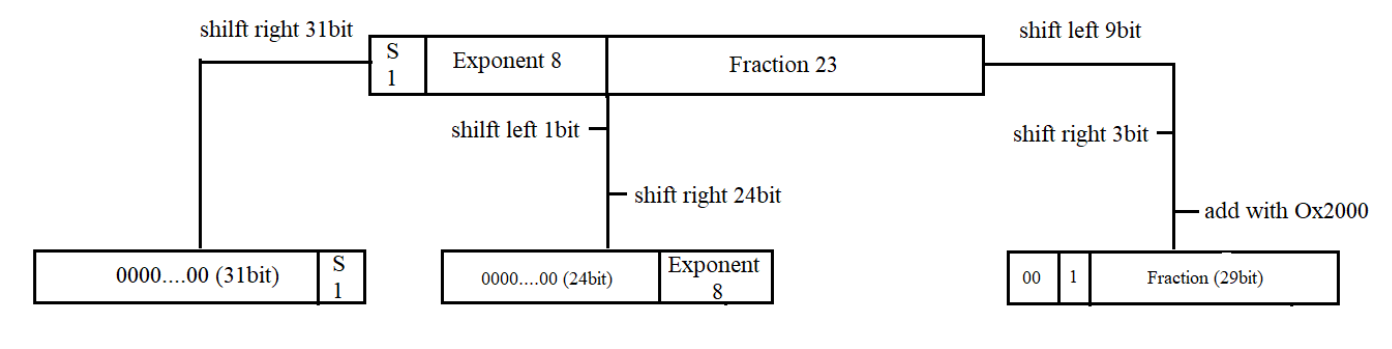
\includegraphics[width=1\textwidth]{image/Mô tả cách lấy thông tin của một số thực trong thanh ghi.png}
         \vspace{0.5cm}
    \caption{Mô tả cách lấy thông tin của một số thực trong thanh ghi}
\end{figure}
\vspace{0.5em}

\noindent \textit{Ghi chú:} 2 bit phụ ở đầu fraction giúp tránh tràn số khi tính toán và hỗ trợ xét dấu sau phép cộng/trừ.

\subsubsection*{2.2.2. Thực hiện phép Cộng/Trừ Hai Thanh Ghi Fraction}
\textbf{Mục tiêu:} Thực hiện phép cộng hoặc trừ giữa hai số thực đã tách và chuẩn hóa, đồng thời xử lý các trường hợp liên quan đến dấu và exponent.\\

\textbf{Quy trình thực hiện}

\begin{enumerate}
    \item \textbf{So sánh Exponent:}  
    Trước khi thực hiện phép cộng hoặc trừ, ta so sánh exponent của hai số thực. Số có exponent nhỏ hơn sẽ được dịch fraction sang phải để căn chỉnh với exponent của số có exponent lớn hơn. Việc dịch bit này sẽ đảm bảo phép toán chính xác trong hệ thống số thực.
    
    \item \textbf{Xử lý Dấu:}  
    Do phần fraction luôn là số dương, ta cần kiểm tra dấu của các thanh ghi. Nếu bit dấu \( S = 1 \), phần fraction của số đó sẽ được đổi dấu (chuyển sang dạng bù 2). Sau khi xử lý dấu, ta có thể tiếp tục thực hiện phép toán cộng hoặc trừ.
    
    \item \textbf{Cộng hoặc Trừ Fraction:}  
    Sau khi đã xử lý dấu và căn chỉnh exponent, ta thực hiện phép cộng hoặc trừ giữa hai phần fraction. Phép cộng được thực hiện như bình thường, còn nếu là phép trừ, ta cần điều chỉnh dấu của một trong các phần fraction.
\end{enumerate}
\subsubsection*{2.2.3. Chuẩn Hóa Kết Quả về Dạng Chuẩn IEEE 754}

\textbf{Mục tiêu:} Đưa kết quả về dạng chuẩn \texttt{1.xxxxxx} như định dạng IEEE 754 yêu cầu.

\begin{enumerate}
    \item Xét dấu kết quả:
    \begin{itemize}
        \item Nếu âm, đặt \texttt{S = 1} và lấy trị tuyệt đối.
        \item Nếu dương, đặt \texttt{S = 0}.
    \end{itemize}
   \item {So sánh với ngưỡng chuẩn IEEE 754:} \\ 
    Để chuẩn hóa kết quả, ta so sánh giá trị với hai ngưỡng chuẩn \( 0x40000000 \) và \( 0x20000000 \):
\begin{itemize}
        \item Nếu kết quả lớn hơn hoặc bằng \( 0x40000000 \), ta thực hiện dịch phải (shift right) để giảm giá trị, đồng thời tăng exponent.
        \item Nếu kết quả nhỏ hơn \( 0x20000000 \), ta thực hiện dịch trái (shift left) để tăng giá trị, đồng thời giảm exponent.
    \end{itemize}
    \item Tiếp tục cho đến khi phần trị nằm trong đoạn $[0x20000000, 0x40000000)$.
     \item Chuyển đổi Fraction:\\  
    Sau khi chuẩn hóa, phần fraction sẽ có dạng \( 1.xxx...xx \) với 30 bit. Điều này đảm bảo rằng phần trị của số thực đã được chuẩn hóa theo chuẩn IEEE 754.
\end{enumerate}

\subsubsection*{2.2.4. Tổ hợp kết quả thành số thực IEEE 754}
\textbf{Mục tiêu:} Tổ hợp các thành phần (dấu \( S \), exponent và fraction) để tạo ra kết quả cuối cùng dưới dạng số thực chuẩn IEEE 754.\\

\textbf{Quy trình thực hiện:}
\begin{enumerate}
    \item Dời các phần vào đúng vị trí:
    \begin{itemize}
        \item \texttt{Dịch phần dấu \( S \) lên bit 31:} \texttt{S << 31}
        \item \texttt{Dịch exponent vào các bit từ 23 đến 30:} \texttt{Exponent << 23}
        \item \texttt{Dịch fraction vào các bit từ 0 đến 22.} 
    \end{itemize}
     Quá trình này giúp tái tạo lại số thực theo định dạng chuẩn IEEE 754.
    \item Tổng hợp kết quả:
       Cuối cùng, kết quả sẽ được lưu vào thanh ghi, sẵn sàng cho các phép toán tiếp theo hoặc xuất ra bộ nhớ.
\end{enumerate}
\begin{lstlisting}
result = (S << 31) | (Exponent << 23) | (Fraction & 0x7FFFFF)
\end{lstlisting}
Hãy xem hình minh họa dưới đây:
\begin{figure}[!h]
    \centering 
    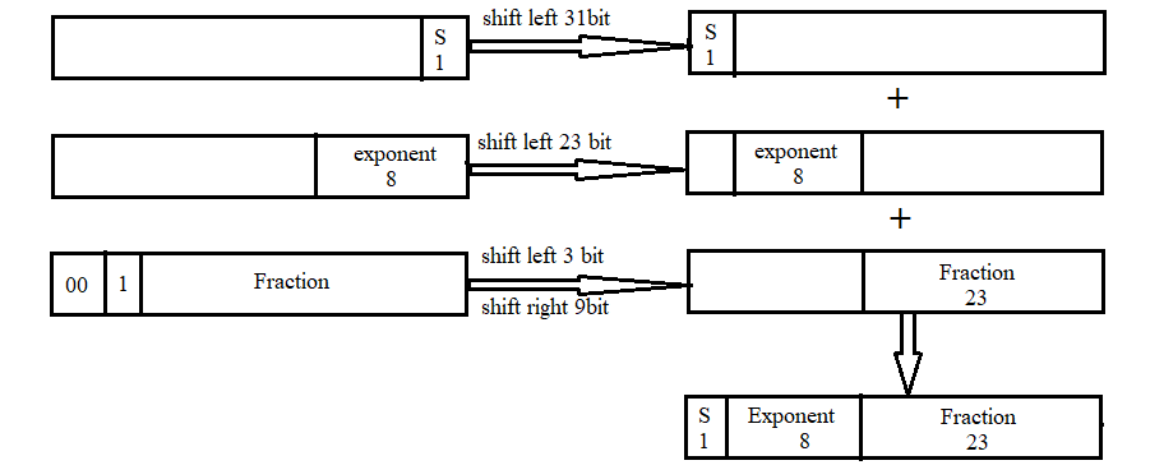
\includegraphics[width=1\textwidth]{image/Tổ Hợp Kết Quả.png}
         \vspace{0.5cm}
    \caption{Mô tả cách lấy thông tin của một số thực trong thanh ghi}
\end{figure}
\vspace{0.5em}
\subsection*{Tổng kết quy trình}
\begin{center}
\begin{tabular}{|l|p{10cm}|}
\hline
\textbf{Giai đoạn} & \textbf{Mô tả} \\
\hline
2.1 & Tách các trường \texttt{S}, \texttt{Exponent}, \texttt{Fraction} từ số thực 32-bit. \\
\hline
2.2 & So sánh số mũ, dịch fraction phù hợp, xử lý dấu và thực hiện phép cộng/trừ. \\
\hline
2.3 & Chuẩn hóa kết quả về dạng chuẩn IEEE 754 bằng dịch bit và điều chỉnh exponent. \\
\hline
2.4 & Tổ hợp các thành phần lại để tạo số thực IEEE 754 chuẩn 32-bit. \\
\hline
\end{tabular}
\end{center}


\section{Chạy code với testcase}
\subsection{Tính thời gian chạy của chương trình}
Thông số hệ thống và giả định:
\begin{itemize}
    \item \textbf{Tần số xung nhịp (Clock Rate)}: 1 GHz ($= 10^9$ chu kỳ/giây)
    \item \textbf{Chu kỳ mỗi lệnh (CPI)}: 1 \\
    \textit{(Giả định: mọi lệnh đều có cùng chi phí thực thi)}
\end{itemize}

\noindent Dựa vào các giả định trên, thời gian thực thi của chương trình được tính theo công thức:

\[
\text{CPU Time} = \frac{\text{Instruction Count} \times \text{CPI}}{\text{Clock Rate}}
\]

Vì CPI = 1, nên công thức rút gọn còn:

\[
\text{CPU Time} = \frac{\text{Instruction Count}}{10^9} \quad \text{(giây)}
\]

\vspace{1em}
Đối với mỗi trường hợp kiểm thử, cần thực hiện:

\begin{enumerate}
    \item Thống kê số lượng và loại lệnh sử dụng (Instruction Types).
    \item Tính toán thời gian thực thi dựa trên tổng số lệnh.
    \item Trình bày kết quả kiểm thử gồm:
    \begin{itemize}
        \item Mô tả chức năng kiểm thử.
        \item Bảng thống kê loại lệnh và số lượng.
        \item Thời gian thực thi tính được.
    \end{itemize}
\end{enumerate}
\vspace{1em}

\noindent \textbf{Nhận xét:} Qua việc phân tích số lượng lệnh và tính toán thời gian thực thi, có thể thấy rằng hiệu năng chương trình phụ thuộc trực tiếp vào số lượng lệnh máy sinh ra. Với giả định CPI = 1 và tần số đồng hồ cố định, việc tối ưu mã nguồn để giảm tổng số lệnh sẽ giúp cải thiện đáng kể thời gian thực thi. Điều này cho thấy tầm quan trọng của việc lựa chọn thuật toán và cấu trúc dữ liệu phù hợp trong quá trình phát triển phần mềm.\\
\newpage

Ta đánh giá hiệu quả của chương trình thông qua một số test cases sau đây:
{\Large
\begin{table}[H]
\centering
\resizebox{\linewidth}{!}{%
% % Phóng to bảng cho vừa toàn bộ chiều ngang trang
\begin{tabular}{|c|c|c|c|c|c|c|c|c|}
\hline
\textbf{a} & \textbf{b} & \textbf{a+b} & \textbf{MIPS} & \textbf{R} & \textbf{I} & \textbf{J} & \textbf{IC} & \textbf{Time (ns)} \\
\hline
3.14 & 4.13  & 7.27  & 7.27 & 56 & 88 & 1 & 145 & 145\\
\hline
3.57 & 2.86 & 6.43  & 6.43 &47 &89 &1 &137 &137 \\
\hline
3.57 & -9.23 & -5.66  &-5.66 &58 &90 &3 &151 & 151\\
\hline
1.0 & 2.0 & 3.0  &3.0 &56 &88 &1 &145 & 145\\
\hline
5.38 & -5.38 & 0.0  &0.0 &41 &82 &2 &125 &125 \\
\hline
5.38 & -10.39 & -5.01  &-5.01 &58 &90 &3 &151 &151 \\
\hline
-321.59 & 555.55 & 233.96  &233.96002 &60 &94 &4 &158 &158 \\
\hline
-55.36 & 123.32 & 67.96  & 67.96 &56 &86 &2 &144 & 144\\
\hline
-578.3612 & 12345.699 & 11767.3378  & 11767.339 &56 & 86& 2&144 & 144\\
\hline
8.12365 & 9.2587 & 17.38235  & 17.382349 &47 &89 &1 &137 &137 \\
\hline
25.032005 & 9.4558 & 34.487805  &34.487804 &47 &89 &1 &137 &137 \\
\hline
-46.8129 & 1427.734&1380.9211   &1380.9211 &56 &86 &2 &144 & 144\\
\hline
-1001.48145 &-1125.919 & -2127.40045 &-2127.4004 &57 &89 &1 &147 &147 \\
\hline
-280.3314 &-11.32654 & -291.65794 &-291.65793 &46 &88 &1 &135 &135 \\
\hline
92656.9 &-20.369747 & 92636.53025 & 92636.53& 46 &86 &2 &134 &134 \\
\hline
3654157.0 &-3651145.8 & 3011.2 &3011.25 &66 &126 &12 &204 &204 \\
\hline
34.232624 &-65.21548 &-30.982856  &-30.982857 & 60 & 94& 4& 158&158 \\
\hline
321.32147 &-1236.5479 & -915.22643 &-915.22644 &58 &90 & 3&151 &151 \\
\hline
680.77045 &-206.09088 &474.67957  &474.67957 & 48 & 90 & 3&141 &141 \\
\hline
-538.9438 &-746.4934 & -1285.4372 &-1285.4371 & 47 & 89 &1 &137 &137 \\
\hline
 -312.01453&-1594.2965 &-1906.31103 &-1906.311 & 56 &88 & 1& 145& 145\\
\hline
-245.30302 &977.04926 &731.74624  & 731.7463&56 & 86&2 &144 & 144\\
\hline
 616.9262&55.415 &672.3412&672.3412 &46 &88 &1 &135 & 135\\
\hline
 46.985474& -1309.58& -1262.594526 &-1262.5945 &56 &86 &2 &144 &144 \\
\hline
 -731.8893&-738.224 &-1470.1133  & -1470.1133&47 &89 &1 &137 & 137\\
 \hline
\end{tabular}
}
\caption{Bảng thống kê kết quả kiểm thử }
\end{table}
}

\subsection{Test case 0:}
\begin{lstlisting}[language=Python]
    a = 3.14;
    b = 4.13;
    a + b = 7.27
\end{lstlisting}

\begin{figure}[!h]
    \centering
    \begin{minipage}[b]{0.48\textwidth}
        \centering
        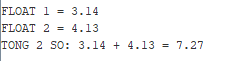
\includegraphics[width=\textwidth]{image/TESTCASE/Testcase 0.png}
    \end{minipage}
    \hfill
    \begin{minipage}[b]{0.48\textwidth}
        \centering
        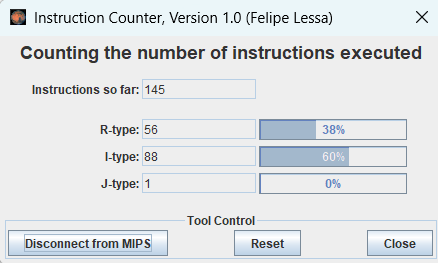
\includegraphics[width=\textwidth]{image/TESTCASE/Instruction Counter 0.png}
    \end{minipage}
    \vspace{0.5cm}
    \caption{Các kết quả kiểm thử cho Testcase 0}
\end{figure}
\[
\text{CPU time} = \frac{\text{145}}{10^9} = 145 ns.
\]

\subsection{Test case 1:}
\begin{lstlisting}[language=Python]
    a = 3.57;
    b = 2.86;
    a + b = 6.43
\end{lstlisting}
\[
\text{CPU time} = \frac{\text{137}}{10^9} = 137 ns.
\]

\begin{figure}[!h]
    \centering
    \begin{minipage}[b]{0.48\textwidth}
        \centering
        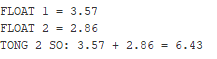
\includegraphics[width=\textwidth]{image/TESTCASE/Testcase 1.png}
    \end{minipage}
    \hfill
    \begin{minipage}[b]{0.48\textwidth}
        \centering
        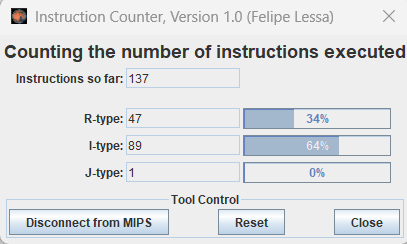
\includegraphics[width=\textwidth]{image/TESTCASE/Instruction Counter 1.png}
    \end{minipage}
    \vspace{0.5cm}
    \caption{Các kết quả kiểm thử cho Testcase 1}
\end{figure}

\vspace{0.5cm}

\subsection{Test case 2:}
\begin{lstlisting}[language=Python]
    a = 3.57;
    b = -9.23;
    a + b = -5.66
\end{lstlisting}
\[
\text{CPU time} = \frac{\text{151}}{10^9} = 151 ns.
\]
\begin{figure}[!h]
    \centering
    \begin{minipage}[b]{0.48\textwidth}
        \centering
        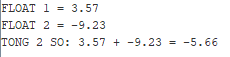
\includegraphics[width=\textwidth]{image/TESTCASE/Testcase 2.png}
    \end{minipage}
    \hfill
    \begin{minipage}[b]{0.48\textwidth}
        \centering
        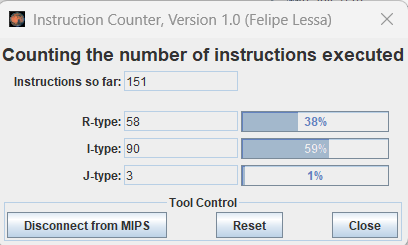
\includegraphics[width=\textwidth]{image/TESTCASE/Instruction Counter 2.png}
    \end{minipage}
    \vspace{0.5cm}
    \caption{Các kết quả kiểm thử cho Testcase 2}
\end{figure}

\vspace{0.5cm}

\subsection{Test case 3:}
\begin{lstlisting}[language=Python]
    a = 1,0;
    b = 2.0;
    a + b = 3.0
\end{lstlisting}
\[
\text{CPU time} = \frac{\text{145}}{10^9} = 145 ns.
\]
\begin{figure}[!h]
    \centering
    \begin{minipage}[b]{0.48\textwidth}
        \centering
        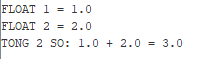
\includegraphics[width=\textwidth]{image/TESTCASE/Testcase 3.png}
    \end{minipage}
    \hfill
    \begin{minipage}[b]{0.48\textwidth}
        \centering
        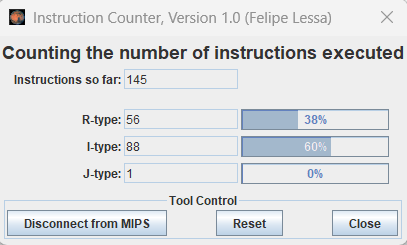
\includegraphics[width=\textwidth]{image/TESTCASE/Instruction Counter 3.png}
    \end{minipage}
    \vspace{0.5cm}
    \caption{Các kết quả kiểm thử cho Testcase 3}
\end{figure}

\vspace{0.5 cm}

\subsection{Test case 4:}
\begin{lstlisting}[language=Python]
    a = 5.38;
    b = -5.38;
    a + b = 0.0
\end{lstlisting}
\[
\text{CPU time} = \frac{\text{125}}{10^9} = 125 ns.
\]

\begin{figure}[!h]
    \centering
    \begin{minipage}[b]{0.48\textwidth}
        \centering
        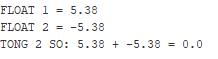
\includegraphics[width=\textwidth]{image/TESTCASE/Testcase 4.png}
    \end{minipage}
    \hfill
    \begin{minipage}[b]{0.48\textwidth}
        \centering
        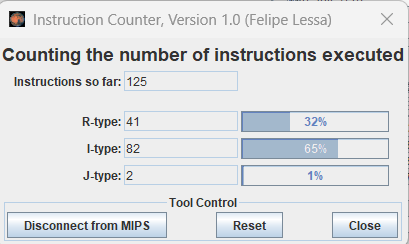
\includegraphics[width=\textwidth]{image/TESTCASE/Instruction Counter 4.png}
    \end{minipage}
    \vspace{0.5cm}
    \caption{Các kết quả kiểm thử cho Testcase 4}
\end{figure}

\vspace{0.5 cm}


\subsection{Test case 5:}
\begin{lstlisting}[language=Python]
    a = 5.38;
    b = -10.39;
    a + b = -5.01
\end{lstlisting}
\[
\text{CPU time} = \frac{\text{151}}{10^9} = 151 ns.
\]
\begin{figure}[!h]
    \centering
    \begin{minipage}[b]{0.48\textwidth}
        \centering
        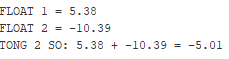
\includegraphics[width=\textwidth]{image/TESTCASE/Testcase 5.png}
    \end{minipage}
    \hfill
    \begin{minipage}[b]{0.48\textwidth}
        \centering
        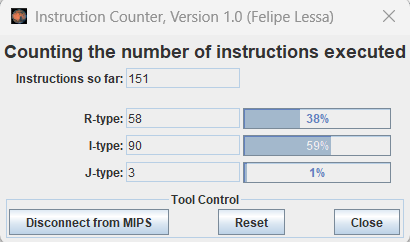
\includegraphics[width=\textwidth]{image/TESTCASE/Instruction Counter 5.png}
    \end{minipage}
    \vspace{0.5cm}
    \caption{Các kết quả kiểm thử cho Testcase 5}
\end{figure}

\vspace{0.5 cm}

\subsection{Test case 6:}
\begin{lstlisting}[language=Python]
    a = -321.59;
    b = 555.55;
    a + b = 233.96
\end{lstlisting}
\[
\text{CPU time} = \frac{\text{158}}{10^9} = 158 ns.
\]
\begin{figure}[!h]
    \centering
    \begin{minipage}[b]{0.48\textwidth}
        \centering
        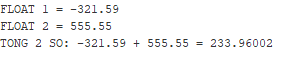
\includegraphics[width=\textwidth]{image/TESTCASE/Testcase 6.png}
    \end{minipage}
    \hfill
    \begin{minipage}[b]{0.48\textwidth}
        \centering
        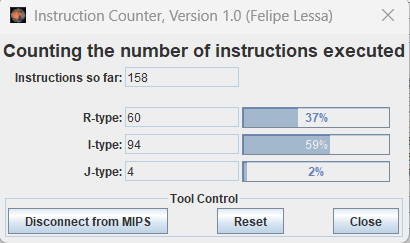
\includegraphics[width=\textwidth]{image/TESTCASE/Instruction Counter 6.png}
    \end{minipage}
    \vspace{0.5cm}
    \caption{Các kết quả kiểm thử cho Testcase 6}
\end{figure}


\vspace{0.5 cm}


\subsection{Test case 7:}
\begin{lstlisting}[language=Python]
    a = -55.36;
    b = 123.32;
    a + b = 67.96
\end{lstlisting}
\[
\text{CPU time} = \frac{\text{144}}{10^9} = 144ns.
\]

\begin{figure}[!h]
    \centering
    \begin{minipage}[b]{0.48\textwidth}
        \centering
        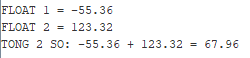
\includegraphics[width=\textwidth]{image/TESTCASE/Testcase 7.png}
    \end{minipage}
    \hfill
    \begin{minipage}[b]{0.48\textwidth}
        \centering
        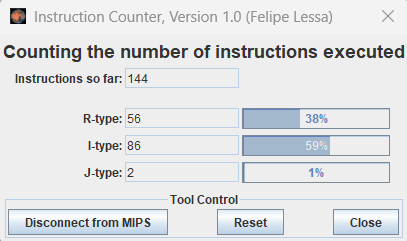
\includegraphics[width=\textwidth]{image/TESTCASE/Instruction Counter 7.png}
    \end{minipage}
    \vspace{0.5cm}
    \caption{Các kết quả kiểm thử cho Testcase 7}
\end{figure}

\vspace{0.5 cm}

\subsection{Test case 8:}
\begin{lstlisting}[language=Python]
    a = -578.3612;
    b = 12345.699;
    a + b = 11767.3378
\end{lstlisting}
\[
\text{CPU time} = \frac{\text{144}}{10^9} = 144ns.
\]
\begin{figure}[!h]
    \centering
    \begin{minipage}[b]{0.48\textwidth}
        \centering
        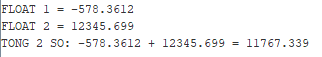
\includegraphics[width=\textwidth]{image/TESTCASE/Testcase 8.png}
    \end{minipage}
    \hfill
    \begin{minipage}[b]{0.48\textwidth}
        \centering
        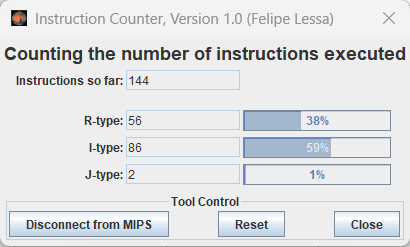
\includegraphics[width=\textwidth]{image/TESTCASE/Instruction Counter 8.png}
    \end{minipage}
    \vspace{0.5cm}
    \caption{Các kết quả kiểm thử cho Testcase 8}
\end{figure}


\subsection{Test case 9:}
\begin{lstlisting}[language=Python]
    a = 8.12365;
    b = 9.2587;
    a + b = 17.38235
\end{lstlisting}


\begin{figure}[!h]
    \centering
    \begin{minipage}[b]{0.48\textwidth}
        \centering
        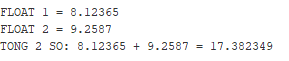
\includegraphics[width=\textwidth]{image/TESTCASE/Testcase 9.png}
    \end{minipage}
    \hfill
    \begin{minipage}[b]{0.48\textwidth}
        \centering
        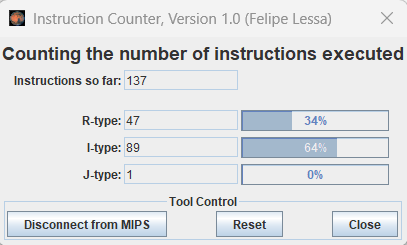
\includegraphics[width=\textwidth]{image/TESTCASE/Instruction Counter 9.png}
    \end{minipage}
    \vspace{0.5cm}
    \caption{Các kết quả kiểm thử cho Testcase 9}
\end{figure}
\[
\text{CPU time} = \frac{\text{137}}{10^9} = 137ns.
\]

\subsection{Test case 10:}
\begin{lstlisting}[language=Python]
    a = 25.032005;
    b = 9.4558;
    a + b = 34.487805
\end{lstlisting}
\[
\text{CPU time} = \frac{\text{137}}{10^9} = 137ns.
\]
\begin{figure}[!h]
    \centering
    \begin{minipage}[b]{0.48\textwidth}
        \centering
        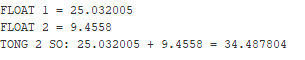
\includegraphics[width=\textwidth]{image/TESTCASE/Testcase 10.png}
    \end{minipage}
    \hfill
    \begin{minipage}[b]{0.48\textwidth}
        \centering
        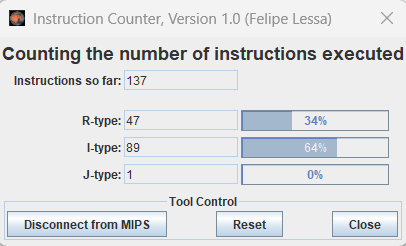
\includegraphics[width=\textwidth]{image/TESTCASE/Instruction Counter 10.png}
    \end{minipage}
    \vspace{0.5cm}
    \caption{Các kết quả kiểm thử cho Testcase 10}
\end{figure}


\vspace{0.5 cm}


\subsection{Test case 11:}
\begin{lstlisting}[language=Python]
    a = -46.8129;
    b = 1427.734;
    a + b = 1380.9211 
\end{lstlisting}
\[
\text{CPU time} = \frac{\text{144}}{10^9} = 144 ns.
\]
\begin{figure}[!h]
    \centering
    \begin{minipage}[b]{0.48\textwidth}
        \centering
        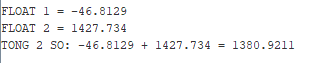
\includegraphics[width=\textwidth]{image/TESTCASE/Testcase 11.png}
    \end{minipage}
    \hfill
    \begin{minipage}[b]{0.48\textwidth}
        \centering
        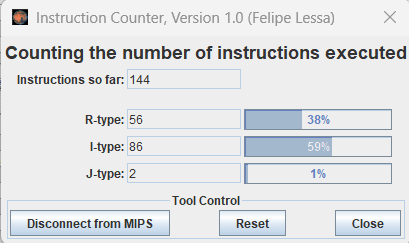
\includegraphics[width=\textwidth]{image/TESTCASE/Instruction Counter 11.png}
    \end{minipage}
    \vspace{0.5cm}
    \caption{Các kết quả kiểm thử cho Testcase 11}
\end{figure}

\vspace{0.5cm}

\subsection{Test case 12:}
\begin{lstlisting}[language=Python]
    a = -1001.48145 ;
    b = -1125.919;
    a + b = -2127.40045
\end{lstlisting}
\[
\text{CPU time} = \frac{\text{147}}{10^9} = 147 ns.
\]
\begin{figure}[!h]
    \centering
    \begin{minipage}[b]{0.48\textwidth}
        \centering
        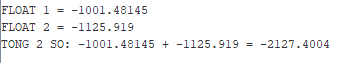
\includegraphics[width=\textwidth]{image/TESTCASE/Testcase 12.png}
    \end{minipage}
    \hfill
    \begin{minipage}[b]{0.48\textwidth}
        \centering
        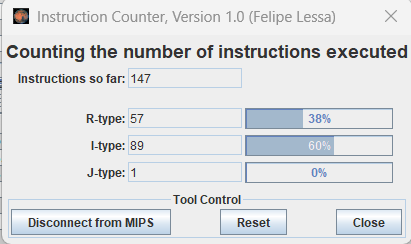
\includegraphics[width=\textwidth]{image/TESTCASE/Instruction Counter 12.png}
    \end{minipage}
    \vspace{0.5cm}
    \caption{Các kết quả kiểm thử cho Testcase 12}
\end{figure}

\vspace{0.5cm}

\subsection{Test case 13:}
\begin{lstlisting}[language=Python]
    a = -280.3314;
    b = -11.32654;
    a + b = -291.65794
\end{lstlisting}


\begin{figure}[!h]
    \centering
    \begin{minipage}[b]{0.48\textwidth}
        \centering
        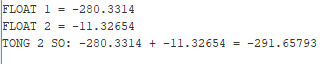
\includegraphics[width=\textwidth]{image/TESTCASE/Testcase 13.png}
    \end{minipage}
    \hfill
    \begin{minipage}[b]{0.48\textwidth}
        \centering
        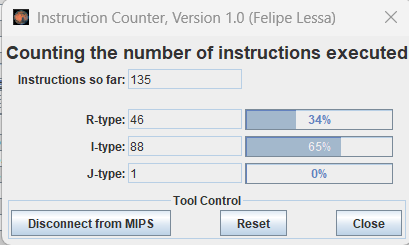
\includegraphics[width=\textwidth]{image/TESTCASE/Instruction Counter 13.png}
    \end{minipage}
    \vspace{0.5cm}
    \caption{Các kết quả kiểm thử cho Testcase 13}
\end{figure}
\[
\text{CPU time} = \frac{\text{135}}{10^9} = 135 ns.
\]

\newpage

\subsection{Test case 14:}
\begin{lstlisting}[language=Python]
    a = 92656.9 ;
    b = -20.369747;
    a + b = 92636.53025
\end{lstlisting}
\[
\text{CPU time} = \frac{\text{134}}{10^9} = 134 ns.
\]
\begin{figure}[!h]
    \centering
    \begin{minipage}[b]{0.48\textwidth}
        \centering
        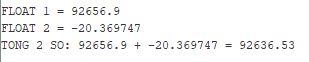
\includegraphics[width=\textwidth]{image/TESTCASE/Testcase 14.png}
    \end{minipage}
    \hfill
    \begin{minipage}[b]{0.48\textwidth}
        \centering
        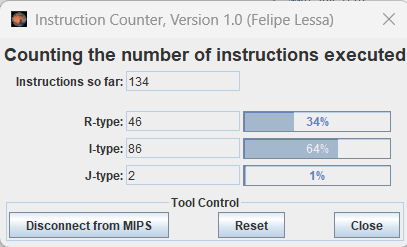
\includegraphics[width=\textwidth]{image/TESTCASE/Instruction Counter 14.png}
    \end{minipage}
    \vspace{0.5cm}
    \caption{Các kết quả kiểm thử cho Testcase 14}
\end{figure}

\vspace{0.5cm}

\subsection{Test case 15:}
\begin{lstlisting}[language=Python]
    a = 3654157.0;
    b = -3651145.8;
    a + b = 3011.2
\end{lstlisting}
\[
\text{CPU time} = \frac{\text{204}}{10^9} = 204ns.
\]

\begin{figure}[!h]
    \centering
    \begin{minipage}[b]{0.48\textwidth}
        \centering
        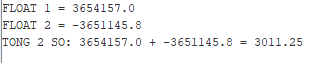
\includegraphics[width=\textwidth]{image/TESTCASE/Testcase 15.png}
    \end{minipage}
    \hfill
    \begin{minipage}[b]{0.48\textwidth}
        \centering
        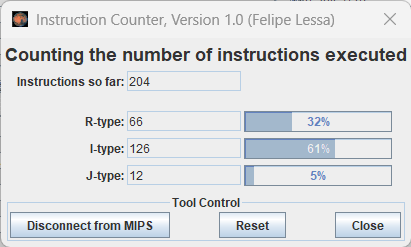
\includegraphics[width=\textwidth]{image/TESTCASE/Instruction Counter 15.png}
    \end{minipage}
    \vspace{0.5cm}
    \caption{Các kết quả kiểm thử cho Testcase 15}
\end{figure}


\newpage
\subsection{Test case 16:}
\begin{lstlisting}[language=Python]
    a = 34.232624;
    b = -65.21548;
    a + b = -30.982856
\end{lstlisting}
\[
\text{CPU time} = \frac{\text{158}}{10^9} = 158 ns.
\]
\begin{figure}[!h]
    \centering
    \begin{minipage}[b]{0.48\textwidth}
        \centering
        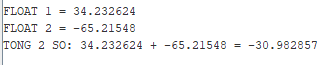
\includegraphics[width=\textwidth]{image/TESTCASE/Testcase 16.png}
    \end{minipage}
    \hfill
    \begin{minipage}[b]{0.48\textwidth}
        \centering
        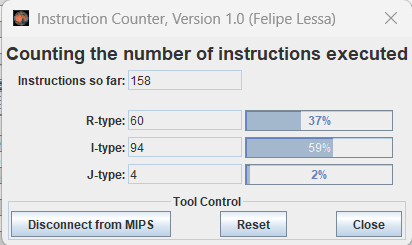
\includegraphics[width=\textwidth]{image/TESTCASE/Instruction Counter 16.png}
    \end{minipage}
    \vspace{0.5cm}
    \caption{Các kết quả kiểm thử cho Testcase 16}
\end{figure}

\subsection{Test case 17:}
\begin{lstlisting}[language=Python]
    a = 321.32147;
    b = -1236.5479;
    a + b = -915.22643
\end{lstlisting}
\[
\text{CPU time} = \frac{\text{151}}{10^9} = 151 ns.
\]

\begin{figure}[!h]
    \centering
    \begin{minipage}[b]{0.48\textwidth}
        \centering
        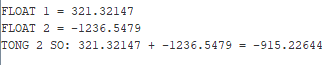
\includegraphics[width=\textwidth]{image/TESTCASE/Testcase 17.png}
    \end{minipage}
    \hfill
    \begin{minipage}[b]{0.48\textwidth}
        \centering
        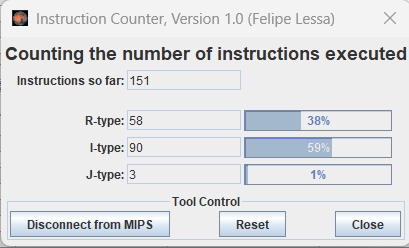
\includegraphics[width=\textwidth]{image/TESTCASE/Instruction Counter 17.png}
    \end{minipage}
    \vspace{0.5cm}
    \caption{Các kết quả kiểm thử cho Testcase 17}
\end{figure}

\subsection{Test case 18:}
\begin{lstlisting}[language=Python]
    a = 680.77045;
    b = -206.09088;
    a + b = 474.67957
\end{lstlisting}
\[
\text{CPU time} = \frac{\text{141}}{10^9} = 141 ns.
\]

\begin{figure}[!h]
    \centering
    \begin{minipage}[b]{0.48\textwidth}
        \centering
        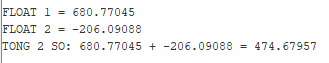
\includegraphics[width=\textwidth]{image/TESTCASE/Testcase 18.png}
    \end{minipage}
    \hfill
    \begin{minipage}[b]{0.48\textwidth}
        \centering
        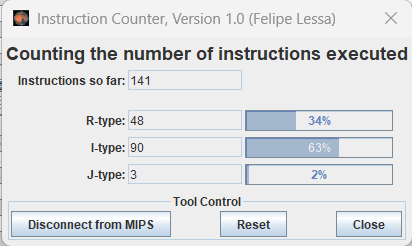
\includegraphics[width=\textwidth]{image/TESTCASE/Instruction Counter 18.png}
    \end{minipage}
    \vspace{0.5cm}
    \caption{Các kết quả kiểm thử cho Testcase 18}
\end{figure}

\vspace{0.5cm}

\subsection{Test case 19:}
\begin{lstlisting}[language=Python]
    a = -538.9438;
    b = -746.4934;
    a + b = -1285.4372
\end{lstlisting}
\[
\text{CPU time} = \frac{\text{137}}{10^9} = 137  ns.
\]

\begin{figure}[!h]
    \centering
    \begin{minipage}[b]{0.48\textwidth}
        \centering
        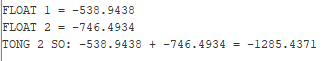
\includegraphics[width=\textwidth]{image/TESTCASE/Testcase 19.png}
    \end{minipage}
    \hfill
    \begin{minipage}[b]{0.48\textwidth}
        \centering
        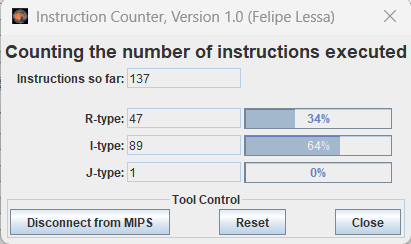
\includegraphics[width=\textwidth]{image/TESTCASE/Instruction Counter 19.png}
    \end{minipage}
    \vspace{0.5cm}
    \caption{Các kết quả kiểm thử cho Testcase 19}
\end{figure}


\subsection{Test case 20:}
\begin{lstlisting}[language=Python]
    a = -312.01453;
    b = -1594.2965;
    a + b = -1906.31103
\end{lstlisting}

\begin{figure}[!h]
    \centering
    \begin{minipage}[b]{0.48\textwidth}
        \centering
        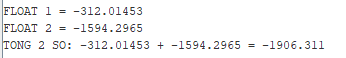
\includegraphics[width=\textwidth]{image/TESTCASE/Testcase 20.png}
    \end{minipage}
    \hfill
    \begin{minipage}[b]{0.48\textwidth}
        \centering
        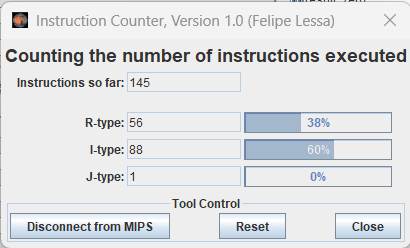
\includegraphics[width=\textwidth]{image/TESTCASE/Instruction Counter 20.png}
    \end{minipage}
    \vspace{0.5cm}
    \caption{Các kết quả kiểm thử cho Testcase 20}
\end{figure}
\[
\text{CPU time} = \frac{\text{145}}{10^9} = 145 ns.
\]

\vspace{0.5cm}

\subsection{Test case 21:}
\begin{lstlisting}[language=Python]
    a = -245.30302;
    b = 977.04926;
    a + b = 731.74624
\end{lstlisting}
\[
\text{CPU time} = \frac{\text{144}}{10^9} = 144  ns.
\]

\begin{figure}[!h]
    \centering
    \begin{minipage}[b]{0.48\textwidth}
        \centering
        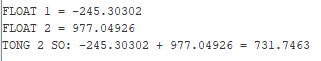
\includegraphics[width=\textwidth]{image/TESTCASE/Testcase 21.png}
    \end{minipage}
    \hfill
    \begin{minipage}[b]{0.48\textwidth}
        \centering
        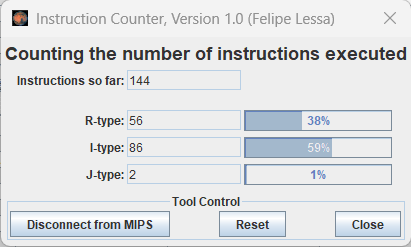
\includegraphics[width=\textwidth]{image/TESTCASE/Instruction Counter 21.png}
    \end{minipage}
    \vspace{0.5cm}
    \caption{Các kết quả kiểm thử cho Testcase 21}
\end{figure}

\vspace{0.5cm}

\subsection{Test case 22:}
\begin{lstlisting}[language=Python]
    a = 616.9262;
    b = 55.415;
    a + b = 672.3412
\end{lstlisting}
\[
\text{CPU time} = \frac{\text{135}}{10^9} = 135 ns.
\]
\begin{figure}[!h]
    \centering
    \begin{minipage}[b]{0.48\textwidth}
        \centering
        \includegraphics[width=\textwidth]{image/TESTCASE/Testcase 22.png}
    \end{minipage}
    \hfill
    \begin{minipage}[b]{0.48\textwidth}
        \centering
        \includegraphics[width=\textwidth]{image/TESTCASE/Instruction Counter 22.png}
    \end{minipage}
    \vspace{0.5cm}
    \caption{Các kết quả kiểm thử cho Testcase 22}
\end{figure}


\subsection{Test case 23:}
\begin{lstlisting}[language=Python]
    a = 46.985474;
    b = -1309.58;
    a + b = -1262.594526
\end{lstlisting}
\[
\text{CPU time} = \frac{\text{144}}{10^9} = 144 ns.
\]
\begin{figure}[!h]
    \centering
    \begin{minipage}[b]{0.48\textwidth}
        \centering
        \includegraphics[width=\textwidth]{image/TESTCASE/Testcase 23.png}
    \end{minipage}
    \hfill
    \begin{minipage}[b]{0.48\textwidth}
        \centering
        \includegraphics[width=\textwidth]{image/TESTCASE/Instruction Counter 23.png}
    \end{minipage}
    \vspace{0.5cm}
    \caption{Các kết quả kiểm thử cho Testcase 23}
\end{figure}


\subsection{Test case 24:}
\begin{lstlisting}[language=Python]
    a = -731.8893;
    b = -738.224;
    a + b = -1470.1133
\end{lstlisting}
\[
\text{CPU time} = \frac{\text{137}}{10^9} = 137 ns.
\]
\begin{figure}[!h]
    \centering
    \begin{minipage}[b]{0.48\textwidth}
        \centering
        \includegraphics[width=\textwidth]{image/TESTCASE/Testcase 24.png}
    \end{minipage}
    \hfill
    \begin{minipage}[b]{0.48\textwidth}
        \centering
        \includegraphics[width=\textwidth]{image/TESTCASE/Instruction Counter 24.png}
    \end{minipage}
    \vspace{0.5cm}
    \caption{Các kết quả kiểm thử cho Testcase 24}
\end{figure}







% \section{Thiết kế ứng dụng}

% \section{Setup Ứng dụng}
% \section{Hiện thực}

% \subsection{Test1}
% a = 5, b =0




\newpage
\addcontentsline{toc}{section}{Tài liệu tham khảo}
\begin{thebibliography}{99999}
\bibitem[1]{1}{Phạm Quốc Cường. } {\em Kiến trúc máy tính}   (3st Edition, 2019), Companion Website:
https://lib.hcmut.edu.vn/kien-truc-may-tinh

\end{thebibliography}
\end{document}